\documentclass[12pt]{article}
\usepackage[utf8]{inputenc}
\usepackage{amssymb,tikz-cd,amsmath,amsthm,enumitem}
\usepackage{color}
\usepackage{tikz}
\usetikzlibrary{shapes.misc,calc,math}
\usetikzlibrary{shapes}
\usetikzlibrary{external}
\tikzset{
vtx/.style={inner sep=2.1pt, outer sep=0pt, circle, fill=blue!50!white,draw=black},
vtx2/.style={inner sep=2.1pt, outer sep=0pt, circle, fill=red!50!white,draw=black},
vtx4/.style={inner sep=3.5pt, outer sep=0pt, circle, fill=blue!50!white,draw=black},
triangle/.style={fill=pink,opacity=0.5,line width=1pt},
novtx/.style={cross out, draw=red, line width=2pt},
gsvtx/.style={inner sep=2.1pt, outer sep=0pt, rectangle, fill=green!50!white,draw=black},
gs2vtx/.style={inner sep=1.8pt, outer sep=0pt, regular polygon,regular polygon sides=5, fill=red!50!white,draw=black},
gs3vtx/.style={inner sep=1.4pt, outer sep=0pt, diamond, fill=yellow!50!white,draw=black},
gs4vtx/.style={inner sep=3.5pt, outer sep=0pt, rectangle, fill=green!50!white,draw=black},
axisedge/.style={-latex, line width=1.5pt},
}

\begin{document}

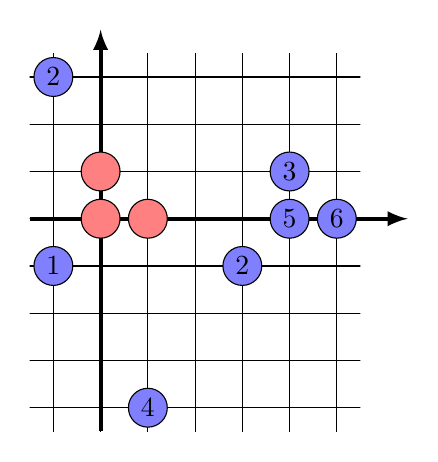
\begin{tikzpicture}[scale=0.6]
   \draw[axisedge] (-1.5,0) -- (6.5,0); 
\draw[axisedge] (0,-4.5) -- (0,4); 
      \clip (-1.5,-4.5) rectangle (5.5,3.5);
      \draw (-2,-5) grid (6,4);
      \begin{scope}[xshift=0cm,yshift=0cm]
         \draw (0,0)node[vtx2]{\phantom{0}};
         \draw (1,0)node[vtx2]{\phantom{0}};
         \draw (0,1)node[vtx2]{\phantom{0}};
         \draw (-1,-1)node[vtx]{1};
         
         \draw (3,-1)node[vtx]{2};
         \draw (-1,3)node[vtx]{2};
         
         \draw (4,1)node[vtx]{3};
         
         \draw (1,-4)node[vtx]{4};
         
         \draw (4,0)node[vtx]{5};
         
         \draw (5,0)node[vtx]{6};
      \end{scope}
   \end{tikzpicture}

\end{document}